\documentclass[10pt,a4paper]{paper}
\usepackage[utf8]{inputenc}
\usepackage{graphicx}
\usepackage{subcaption}
\usepackage{enumitem}
\usepackage{tikz}
\usetikzlibrary{calc}
\usepackage{pgfgantt}
\definecolor{TableOrange}{RGB}{255,151,46}
\definecolor{TableBlue}{RGB}{38,125,184}

\newcommand{\tup}[1]{{\langle #1 \rangle}}

\pdfoptionpdfminorversion=5


\title{Artificial Intelligence for the Automated Synthesis and Validation of Programs}
\author{Sergio Jim\'enez Celorrio\\
\footnotesize Universitat Politècnica de València, Spain\\
\small Area: \underline{Ciencias de la Computación y Tecnología Informática}}

\begin{document}
\maketitle

\begin{abstract}
  Programming is still a manual handcraft task, even when the complexity of programs is not high enough to justify the cost of the human workforce to produce them. The need to automate programming tasks increases every day: Programming errors, commonly known as {\em bugs}, cause undesired software behavior making programs crash or enabling malicious users to access private data. Just for 2017, the cumulative cost of software bugs is worldwide estimated in more than one trillion US dollars. 

  This research project investigates a novel approach for software development, that leverages Artificial Intelligence, to increase the automation of the programming process and hence, reduce the chances of introducing software bugs. The project proposes to address {\bf automatic program synthesis and validation starting from {\em input-output} tests cases, and using {\em AI planning} as a problem solving engine}. Our current work on this particular research topic is the recipient of the {\em 2016 distinguished paper award} at {\sc IJCAI}, the main international conference on Artificial Intelligence.
\end{abstract}

\newpage

\section{Historial científico-técnico del Equipo de Investigadores (Apartado 5.1,bases de la convocatoria)}

The project will be developed within the {\em Group of Reasoning on Planning and Scheduling} (GRPS, {\tt http://users.dsic.upv.es/grupos/grps/}), that is part of the {\em Department of Computer Systems and Computation} of the UPV (DSIC, {\tt www.dsic.upv.es}).

In the last 10 years, the GRPS has led three research projects of the Spanish national research plan on {\em AI planning}. Further, the GRPS has developed its own AI planner, that is participating  at the International Planning Competition (IPC-2018, {\tt https://ipc2018.bitbucket.io}).

The research group for this project comprises three researchers: 1 principal investigator, 1 senior researcher and 1 PhD student. All of them are GRPS members. 

\subsection{Principal Investigator: Sergio Jiménez Celorrio}
Sergio is a {\em Ramón y Cajal} fellow at the Universitat Politècnica de València (2017-2022). Previously, Sergio was a post-doc at the University of Melbourne and a {\em Juan de la Cierva} fellow at the Universitat Pompeu Fabra de Barcelona. From 2004 to 2013 Sergio was assistant lecturer at the Universidad Carlos III de Madrid where he obtained the {\em Distinguished Thesis Award 2011}. Sergio is co-organizer of the {\em $7^{th}$ International Planning Competition} and program committee at top international conferences on Artificial Intelligence (including ICAPS that is the main international conference on {\em AI planning}).

His research addresses complex {\em decision-making} problems with innovative integrations of two {\em Artificial Intelligence} paradigms: {\em Machine Learning} and {\em AI Planning}. His research trajectory on this topic has produced a novel approach to the synthesis of programs, grammars and controllers for autonomous behavior and is the recipient of the {\it 2016 distinguished paper award} at the International Joint Conference on Artificial Intelligence (IJCAI)\footnote{IJCAI is ranked as {\it A+} by the CORE rank and with {\it h5-index} 43 at Google Scholar}, the main international conference on {\em Artificial intelligence}.

His top five scientific contributions are:
\begin{enumerate}
\item Inductive programming with AI planning{\footnotesize~\cite{javi-ijcai17},~\cite{segovia2016generalized},~\cite{jimenez2015computing}}.
\item Generalization in AI planning{\footnotesize~\cite{javi-icaps17},~\cite{damir-derived-ijcai16},~\cite{javi-fsc-ijcai16}}.
\item Learning to relieve the {\it knowledge acquisition bottleneck} in AI planning{\footnotesize{~\cite{diego-icaps18},~\cite{jimenez2013integrating},~\cite{jimenez2008architecture},~\cite{jimenez2006planning},~\cite{lanchas2007learning}}}.
\item Machine learning for addressing the {\it curse of dimensionality} in AI planning{\footnotesize~\cite{jimenez2012review},~\cite{de2011scaling},~\cite{de2008learning}}.  
\item Evaluation in AI planning{\footnotesize~\cite{lopez2015deterministic},~\cite{lopez2013automating},~\cite{coles2012survey}}. 
\end{enumerate}

\underline{General quality indicators of scientific research}: {\bf 381 citations} (295 since 2013) and {\bf h-index 11}. {\scriptsize\em Source google scholar}.


\subsection{Senior Researcher: Eva Onaindia}
Eva Onaindia is a {\em Full Professor} at the Universitat Politècnica of València. She leads the GRPS where she conducts research in Artificial Intelligence, Automated Planning, Causal Model Learning and Recommender Systems.

Eva has published numerous articles in top-tier specialized conferences such as the International Joint Conference on Artificial Intelligence (IJCAI), Autonomous Agents and Multi Agent Systems (AAMAS), International Conference on Planning and Scheduling (ICAPS) or European Conference on Artificial Intelligence (ECAI), among others; and scientific journals related to topics of Artificial Intelligence, Planning, Argumentation and Recommender Systems such as IEEE Intelligent Systems, Information Sciences, Engineering Applications of Artificial Intelligence, Knowledge and Information Systems or Applied Intelligence, among others.

She has led several projects from the {\em National research plan} as well as served on multiple ICAPS, AAAI, IJCAI and ECAI conferences as a member of the Program Committee and as a senior member. Eva is Editor-in-Chief of the journal AI Communications, a Review Board member of the journal Applied Intelligence and she will be Program co-chair of ICAPS 2019 (the main international conference on AI planning). 

Eva Onaindía has supervised so far a total of nine PhD theses and she currently supervising four doctoral students. She has also participated in many diverse scientific evaluation committees at both national and international level. In the national scene, she has collaborated with National agencies ANEP and ANECA and she has been member of different expert boards and scientific committees. At an international level, she has participated in the evaluation of research projects for Israel, Italy or Czech Republic.

Eva has also participated in several R\&D and Innovation contracts: with the firm {\sc DESTINIA S.L.} ({\tt https://destinia.com/}) for the development of a tourist recommender system, and currently in the construction of a system for {\em electricity price forecasting} aimed at energy savings (Ayuntamiento Lliria) using neural networks and data analysis techniques.

\underline{General quality indicators of scientific research}: {\bf 1532 citations} (989 since 2013) and {\bf h-index 22}. {\scriptsize\em Source google scholar}.


\subsection{Researcher in training period: Diego Aineto}
Diego Aineto is a PhD student at the {\em Department of Computer Systems and Computation} of the UPV.

Since 2016 Diego is holding a four-year FPU grant on {\em Causal discovery for predictive analysis} (FPU16/03184). Diego is also involved on the current research project TIN2017-88476-C2-1-R of the GPRS from the Spanish national research plan with title {\small\em RECONOCIMIENTO DE ACTIVIDADES Y PLANIFICACION AUTOMATICA PARA EL DISEÑO DE ASISTENTES INTELIGENTES}.

With Eva Onaindia and Sergio Jiménez, Diego is already co-author of one paper on the International Conference on Planning and Scheduling (ICAPS)~\cite{diego-icaps18}, and one journal paper~\cite{onaindia2018common}. Both papers on research topics related to the development of this project. 


\newpage
\section{Estado del arte y objetivos específicos ( Apartado 5.2.i, bases de la convocatoria)}

This research project will {\bf investigate the integration of {\em AI planning} into the {\em Test Driven Development} paradigm for the automatic synthesis and validation of programs}. Here we briefly introduce the technology we will rely on along the project:
\begin{itemize}
\item {\bf AI Planning (AIP)} is the Artificial Intelligence component that studies the synthesis of sets of actions to achieve some given objectives~\cite{ghallab2004automated}. AIP arose in the late ’50s from converging studies into {\em combinatorial search}, {\em theorem proving} and {\em control theory} and now, is a well formalized paradigm for problem solving with algorithms that scale-up reasonably well. State-of-the-art planners are able to synthesize plans with hundreds of actions in seconds time~\cite{geffner2013concise}.  The mainstream approach for AIP is {\em heuristic search} with heuristics derived automatically from the problem representation~\cite{mcdermott1996heuristic,bonet2001planning}.  Current planners add other ideas to this like {\it novelty exploration}~\cite{geffner:psimulators:IJCAI17}, {\it helpful actions}~\cite{hoffmann2001ff}, {\it landmarks}~\cite{helmert2006fast}, and {\it multiqueue best-first search}~\cite{richter2010lama} for combining different heuristics.
  
\item {\bf Test driven development (TDD)}~\cite{beck:TDD:2003} is a popular paradigm for software development that is frequently used in {\it agile methodologies}~\cite{cohen2003agile}. In TDD, test cases are created before the program code is written and they are run against the code during the development, e.g. after a code change via an automated process. When all tests pass, the program code is considered {\em complete} while when a test fails, it pinpoints a {\em bug} that must be fixed from the program code. Tests cases are a natural form of program specification, programmers often claim {\em 'code that is difficult to test is poorly written'}. Further, tests alert programmers of bugs before handing the code off to clients (the cost of finding a bug when the code is first written is considerably lower than the cost of detecting and fixing it later). %Last but not least, writing a thorough set of tests cases forces programmers to think through inputs, outputs, and error conditions of programs. 
\end{itemize}

{\em Program synthesis} is the task of computing a program that satisfies a given formal specification. The 2008 PhD Thesis work by Armando Solar-Lezama, at the University of California Berkeley, showed that it is possible to encode program synthesis problems in Boolean logic and therefore, use SAT algorithms to automatically compute programs~\cite{lezama2008program}. Since then, there has been a surge of practical interest in the idea of program synthesis in the formal verification community and related fields~\cite{alur2013syntax}. To illustrate this, in 2013, a unified framework for program synthesis problems was proposed and since 2014 there is a yearly program synthesis competition, comparing the different algorithms for program synthesis in a competitive event ({\tt www.sygus.org}).

Now we review the two most successful approaches for automated program synthesis. 
\begin{itemize}
\item{\bf Programming by Example (PbE)}. PbE techniques have already been deployed in the real world and are part of the {\sc Flash Fill} feature of Excel in Office 2013 that generates programs for string transformation~\cite{gulwani2011automating}. In this case the set of synthesized programs are represented succinctly in a restricted Domain-Specific Language (DSL) using a data-structure called version space algebras~\cite{mitchell1982generalization}. The programs are computed with a domain-specific search that implements a divide and conquer approach. 

\item In {\bf Programming by Sketching (PbS)} programmers provide a partially specified program, i.e.~a program that expresses the high-level structure of an implementation but that leaves low level details undefined to be determined by the synthesizer~\cite{solar2006combinatorial}. This form of program synthesis relies on a programming language called {\sc SKETCH}, for sketching partial programs. PbS implements a counterexample-driven iteration over a synthesize-validate loop built from two communicating SAT solvers, the inductive synthesizer and the validator, to automatically generate test inputs and ensure that the program satisfy them. Despite, in the worst case, program synthesis is harder than NP-complete, this counterexample-driven search terminates on many real problems after solving only a few SAT instances~\cite{lake2015human}.
\end{itemize}

The synthesis of {\it Finite State Controllers} (FSCs)~\cite{geffner:policies:IJCAI15} is closely related to program synthesis. The state-of-the-art algorithms for computing FSCs follow a {\it top-down} approach that interleaves {\it programming} the FSC with validating it~\cite{sergio:aprograming:ijcai16}. To keep the computation of FSCs tractable, they limit the space of possible solutions bounding the maximum size of the FSC. The computation of FSCs includes works that compile this task into another forms of problem solving so they benefit from the last advances on off-the-shelf solvers (e.g. {\em classical planning}~\cite{sergio:aprograming:icaps16}, {\em conformant planning}~\cite{Geffner:FSM:AAAI10}, {\em CSP}~\cite{Infantes:FSC:ECAI2010} or a {\em Prolog program}~\cite{Giacomo:FSM:ICAPS13}). The generation of programs from examples is a research question also addressed in the classic AI field of {\em Inductive Logic Programming} (ILP)~\cite{muggleton1991inductive,Raedt:relationalML:book2008}. ILP arises from the intersection of {\em Machine Learning} and {\em Logic Programming} and deals with the development of inductive techniques to learn a given target concept, expressed as a  logic program,  from  examples  and  background  knowledge, that are expressed as logic facts.

On the other hand, {\em program validation} is the task of proving, or disproving, the correctness of a given program with respect to a certain formal specification or property. Program validation is considered a necessary step for program synthesis. {\em Model checking} is the best-known approach for program validation~\cite{clarke1999model}. In model checking a given model of a system, is exhaustively and automatically checked to verify  whether this model meets a given specification. Typically the specification contains safety requirements such as the absence of deadlocks and similar critical states that can cause the system to crash. Both the model of the system and the specification are formulated in a formal language. To this end, the problem is formulated as a task in logic, namely to check whether a given structure satisfies a given logical formula. 

Currrent approaches for model checking reduces to graph search. Instead of enumerating reachable states one at a time, the state space can sometimes be traversed more efficiently by considering large numbers of states at a single step. When such state space traversal is based on representations of set of states and transition relations as logical formulas, binary decision diagrams (BDD) or other related data structures, the model-checking method is symbolic~\cite{mcmillan1993symbolic}.


\begin{center}
{\small (Please find the full list of {\em references} at the end of the document)}
\end{center}

\newpage
\section{Metodología y Plan de Trabajo ( Apartado 5.2.ii, bases de la convocatoria)}
\label{subsec:metodologia}
Our current research already shows that AI planners can synthesize programs for non trivial tasks like sorting lists, traversing graphs or manipulating strings~\cite{jimenez2015computing,sergio:aprograming:icaps16,sergio:aprogramingb:ijcai16,sergio:aprograming:ijcai16}. Table~\ref{tab:programs} reports the time invested by the AI planner {\sc FD}~\cite{helmert2006fast} to solve the following programming tasks: computing the $n^{th}$ term of the {\em summatory} and  {\em Fibonacci} series, {\em reversing} a list, {\em finding} an element (and the {\em minimum} element) in a list, {\em sorting} a list and traversing a binary tree. 
 
\begin{table*}[hbt!]
  \centering
\begin{small}  
\begin{tabular}{l@{\hspace*{30pt}}c@{\hspace*{5pt}}}
 \textbf{Programming Task} & \textbf{Time (seconds)} \\\hline
Summatory		&	1\\
Fibonacci		&	5\\
Reverse			&	22\\
Find                    &       336 \\
Minimum                 &       284 \\
Sorting			&	30\\
Tree  		&	165
\end{tabular}
\end{small}  
\caption{\small Time to synthesize the programs with the AI planner {\sc FD}~\cite{helmert2006fast} on a processor {\em Intel Core i5 3.10GHz x 4} and with a 4GB memory bound.}
\label{tab:programs}
\end{table*}

\subsection{Synthesis and validation of TDD programs as AI planning}
Given a {\em TDD programming} task our approach is modeling and solving it as it were an {\em AI planning} task.

Briefly the {\bf state variables} of this AIP task are {\em fluents} of the kind:
\begin{itemize}
\item {\tt var:=value}, that encode the program variables.
\item {\tt program(line):=instruction}, that encode the instructions at the different program lines.
\item {\tt pcounter:=line}, encoding the current program line.
\end {itemize}

The {\bf initial/goal states} of the AIP task encode the initial/final values of the program variables that are given by the input/output tests of the TDD programming task.

Finally, program instructions are encoded using two kinds of AIP {\bf actions}:
\begin{itemize}
\item {\it Programming actions}, that set an instruction on a given program line.
\item {\it Execution actions}, execute the instruction set on a given program line.
\end{itemize}
We implement this encoding using standard planning languages, such as PDDL~\cite{fox2003pddl2}, so the AIP tasks resulting from our encoding can be solved with off-the-shelf planners, like {\sc FD}~\cite{helmert2006fast}. The programs synthesized with this approach are guaranteed to be bug-free over given sets of {\em input-output} tests cases.

Interestingly, our PDDL encoding allows also program validation by (1), specifying the lines of the program to validate (i.e. the {\tt program(line):=instruction} fluents) in the initial state of the AIP task and (2), disabling the mentioned {\it programming actions} so only {\it execution actions} are applicable. 

\subsection{Evaluation}
\label{sec:evaluation}
The performance of our approach for the synthesis and validation of TDD programs will be evaluated in two kinds of programming tasks:
\begin{itemize}
\item {\em Real-world benchmarks}: The GRPS group is currently leading a four-year research project from the {\em Spanish national plan} in which {\em activity recognition} is applied to different real-world domains such as {\em domotics}, {\em tourism}, {\em traffic control} and {\em robotics}. Interestingly many activities in these domains can be understood as simple programs. For instance, Figure~\ref{fig:activity} shows a four-line program (pictured as a finite state machine) that represents the sequence of instructions required for the {\em making a buttered toast} activity. We plan to evaluate our approach in synthesis and validation tasks coming from these real-world domains. 

\begin{figure}[hbt!]
\begin{center}
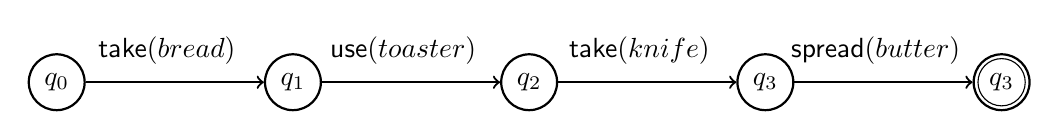
\begin{tikzpicture}
\node [thick,draw,circle] at (1,1.1) (x) {$q_0$};
\node [thick,draw,circle] at (4,1.1) (y) {$q_1$};
\node [thick,draw,circle] at (7,1.1) (v) {$q_2$};
\node [thick,draw,circle] at (10,1.1) (w) {$q_3$};
\node [thick,draw,circle] at (13,1.1) (z) {$q_3$};
\draw (13,1.1) circle (.3cm);

\draw [thick,->] (x) to (y);
\draw [thick,->] (y) to (v);
\draw [thick,->] (v) to (w);
\draw [thick,->] (w) to (z);

\node at (2.4,1.5) {$\mathsf{take}(bread)$};
\node at (5.4,1.5) {$\mathsf{use}(toaster)$};
\node at (8.4,1.5) {$\mathsf{take}(knife)$};
\node at (11.4,1.5) {$\mathsf{spread}(butter)$};

\end{tikzpicture}
\end{center}
\caption{\small Four-line program representing the activity of {\em making a buttered toast}.}
\label{fig:activity}
\end{figure}


\item {\em Theoretical benchmarks}: Classic programming tasks are a neat touchstone to assess the performance of our approach. For instance, programs for the computation of mathematical/logic series, string manipulation and for the management of data structures such as {\em lists}, {\em queues}, {\em stacks} or {\em trees}. Figure~\ref{fig:list} shows a synthesized program for traversing a linked list. The program is pictured as a {\em finite state machine}: The machine nodes mount to the different program lines while edges are tagged with a {\em condition/instruction} label, that denotes the condition (over the program variables) under which program instructions are taken.  
\end{itemize}


\begin{figure}[hbt!]
\begin{center}
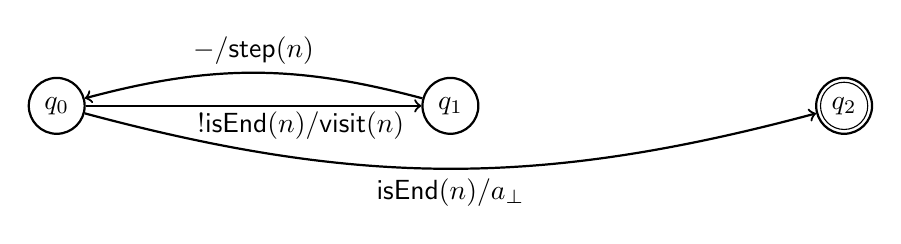
\begin{tikzpicture}
\node [thick,draw,circle] at (1,1.1) (x) {$q_0$};

\node [thick,draw,circle] at (6,1.1) (y) {$q_1$};

\node [thick,draw,circle] at (11,1.1) (z) {$q_2$};

\draw (11,1.1) circle (.3cm);

\draw [thick,->] (x) -- (y);

\draw [thick,out=345,in=195,->] (x) to (z);

\draw [thick,out=165,in=15,->] (y) to (x);

\node at (4.1,0.85) {$!\mathsf{isEnd}(n)/\mathsf{visit}(n)$};
\node at (3.5,1.8) {$-/\mathsf{step}(n)$};
\node at (6,0) {$\mathsf{isEnd}(n)/a_\bot$};
\end{tikzpicture}
\end{center}
\caption{\small Synthesized program to solve the programming task of traversing a linked list ($n$ is a variable that points to a node of the linked list).}
\label{fig:list}
\end{figure}


%The space of the possible programs encoded in such a way grows exponentially in the number of possible program lines. To address challenging tasks our approach must then be combined with {\em problem decomposition}. With this regard, our encoding supports callable procedures to decompose a given programming task in simpler modules and to enable recursive solutions~\cite{sergio:aprograming:icaps16,sergio:aprograming:ijcai16}. 

\subsection{Workplan}
We designed a 24-month workplan plan for the {\bf development of a user-interactive program synthesizer} that (1), takes as input a set of test cases that specify the TDD programming task to solve and (2), outputs a program source code that passes these tests with a bug-free guarantee.

In the particular case that the {\em program synthesizer} receives an additional input specifying the program source code, it outputs a validation certificate guaranteeing that the input program passes the given test cases. Figure~\ref{fig:gantt} details the proposed 24-month timeline for the project.

\begin{figure}[hbt!]
\begin{ganttchart}[
  hgrid,
  group progress label node/.append style={below=3pt},
  canvas/.append style={label=below:} ]{1}{12} 
\ganttbar[bar/.append style={line width=1pt, draw=TableBlue,fill=TableBlue,fill opacity=0.6274509804}]{Design (6 months)}{1}{3} \\
\ganttbar[bar/.append style={line width=1pt, draw=TableBlue,fill=TableBlue,fill opacity=0.6274509804}]{Development (6 months)}{4}{6}\\
\ganttbar[bar/.append style={line width=1pt, draw=TableBlue,fill=TableBlue,fill opacity=0.6274509804}]{Experiments \& dissemination (12 months)}{7}{12}
\end{ganttchart}
\caption{\small Work-plan for developing a user-interactive program synthesizer/validator.}
\label{fig:gantt}
\end{figure}


\begin{enumerate}
\item {\bf T1. System design (months 1-6})
  \begin{small}
    \begin{enumerate}
    \item Design of the user-interaction for the test-case specification. Programming tasks are specified as a set of {\em input-output} tests cases plus the available instruction set. 
    \item Experimental design. Experiments will comprise taking time and memory measurements to evaluate the resources required by our approach to solve the given TDD programming/validation tasks.
      \item Evaluation of different AI planners available, with special attention to the planners that get the best results at the IPC-2018. 
      \end{enumerate}
  \end{small}

{\small{\bf\em  Deliverable T1:} Technical report with the specifications of the system design.}
  
  \item {\bf T2. Development of the system architecture (months 7-12})
    \begin{small}
      \begin{enumerate}
      \item The programming-into-planning compiler ({\em Compiler 1}). This component parses the {\em TDD programming task} and produces an {\em AIP task} encoded in the standard planning language PDDL.
      \item The plan-into-program compiler ({\em Compiler 2}). This component extracts the program code and the corresponding validation certificate from the solution plan produced by an off-the-shelf AI planner.
      \end{enumerate}
\end{small}      

\begin{figure}[hbt!]
\tikzstyle{block} = [draw, draw=TableBlue,fill=TableBlue,fill opacity=0.6274509804, rectangle, minimum height=3em, minimum width=6em]
\tikzstyle{input} = [coordinate]
\tikzstyle{output} = [coordinate]
\begin{center}
\begin{tikzpicture}[auto, node distance=2cm,>=latex']
    % We start by placing the blocks
    \node [input, name=input] {};
    \node [block, right of=input, node distance=4cm] (compiler1) {Compiler 1};
    \node [block, below of=compiler1, node distance=2cm] (planner) {AI Planner};    
    \node [block, below of=planner, node distance=2cm] (compiler2) {Compiler 2};
    \node [output, right of=compiler2, node distance=3cm] (output) {Program};


    % Once the nodes are placed, connecting them is easy. 
    \draw [->] (input) -- node {Programming task} (compiler1);
    \draw [->] (compiler1) -- node[] {AIP task} (planner);
    \draw [->] (planner) -- node[] {Solution plan} (compiler2);        
    \draw [->] (compiler2) -- node[] {Program}(output);
\end{tikzpicture}
\end{center}  
\caption{\small System architecture for the synthesis and validation of TDD programs.}
\label{fig:architecture}
\end{figure}

{\small{\bf\em Deliverable T2:} Open repository with the source code of the system architecture.}
    
\item {\bf T3. Experiments and dissemination of results (months 13-24}).
   \begin{small}
      \begin{enumerate}
      \item Reporting the experimental performance of our AIP approach for solving diverse TDD programming tasks. This task will follow an iterative workflow over the following subtasks:
      \begin{enumerate}
      \item Executing the system architecture in the {\em theoretical benchmarks} described in Section~\ref{sec:evaluation}.
      \item Analysis and validation of the obtained results.
      \item Tuning and repairing the system components, evaluation metrics and benchmarks according to the obtained results.                 
      \item Executing the system architecture in the {\em real-world benchmarks} introduced in Section~\ref{sec:evaluation}.
      \item Analysis and validation of the obtained results.         
      \item Tuning and repairing the system components, evaluation metrics and benchmarks according to the obtained results.                 
      \end{enumerate}
      \item Dissemination of the obtained theoretical and empirical results by submitting papers to top international conferences and journals in AI.        
      \end{enumerate}
\end{small}        
{\small{\bf\em  Deliverable T3:} Final report with the obtained conclusions and produced publications.}
\end{enumerate}

\subsection{Workload}

{\em Tasks ({\bf T1-T3})} will be developed by the three mentioned members of the research group: Sergio Jiménez, Eva Onaindia and Diego Aineto.

In addition, we plan to hire a master student to assist in the completion of two tasks, {\bf T3(a,i)} and {\bf T3(a,iv)}. His detailed responsability will be:
\begin{enumerate}
\item Executing the scripts of the system architecture.
\item Collecting the output data.
\item Presenting the output data in a easy-readable format.
\end{enumerate}

\newpage
\section{Objetivos específicos del Proyecto ( Apartado 5.2.iii, bases de la convocatoria)}
\label{subsec:objectivos}

The objective of this project is to study the performance of our approach for the automated synthesis and validation of programs that are characterized by these tree dimensions:
\begin{enumerate}
\item Number of {\em program lines}.
\item Number and domain of the observable {\em program variables}.
\item Size of the available {\em instruction set}.
\end{enumerate}  

For instance, the program of Figure~\ref{fig:list} is generated using three program lines, one observable variable ($\mathsf{isEnd}(n)$ that has Boolean domain and indicates when $n$ points to the end of the linked list), and a instruction set that comprises two instructions ($\mathsf{visit}(n)$ that marks the list node assigned to $n$ as {\em visited} and $\mathsf{step}(n)$ that advances $n$ to the next node in the linked list).

In more detail, the two specific objectives of this project are:
\begin{itemize}
\item To study the performance of our Artificial Intelligence approach for the {\bf synthesis of programs} up to: {\bf 10 program lines}, {\bf 10 observable variables} with binary domain and, an instruction set that comprises {\bf 10 instructions}. 
\item To study the performance of our Artificial Intelligence approach for the {\bf validation of programs} up to: {\bf 15 program lines}, {\bf 15 observable variables} with binary domain and, an instruction set that comprises {\bf 15 instructions}. 
\end{itemize}
In both cases the performance of our approach will be evaluated with regard to the {\bf computation time} and {\bf memory} invested in the synthesize and the validation of the aimed programs.

Despite setting bounds for the programs size and kind, note that challenging programming tasks can be addressed using {\em problem decomposition}. With this regard, our AIP encoding already supports callable procedures to decompose a given programming task into simpler modules and to enable recursive solutions~\cite{sergio:aprograming:icaps16,sergio:aprograming:ijcai16}.


\newpage
\section{Beneficios del proyecto. Difusión y Explotación en su caso de los Resultados.}
\label{subsec:beneficios}
AIP has recently shown successful in {\em program testing} to generate {\em attack plans} that completed non-trivial software security tests~\cite{hoffmann2015simulated,steinmetz2016revisiting,shmaryahu2016constructing,steinmetz2016goal}. Promising research opportunities come from the application of AIP to {\em program synthesis} given that, {\em program synthesis} with a tests base, can be seen as the {\em program testing} dual.

In fact, our current work on {\em program synthesis} with AIP already produced {\bf publications at top international conferences on Artificial Intelligence}~\cite{segovia2017generating,sergio:aprogramingb:ijcai16,sergio:aprograming:ijcai16,sergio:aprograming:icaps16} and is the recipient of the {\it 2016 distinguished paper award} at the International Joint Conference on Artificial Intelligence, the main international conference on {\em Artificial intelligence}. 

In more detail, the expected benefits for this particular research project are four-fold:
\begin{enumerate}
\item The definition of {\bf effective metrics for assessing how well a given program covers a set of {\em input-output} test cases}. These metrics can provide new insights into the current understanding of how Artificial Intelligence can assist programmers in the software development. 
\item An empirical {\bf study on the performance of the state-of-the-art AI planners for the {\em Synthesis and Validation of Programs}}. Research in AI algorithms is too often tested with laboratory problems and AIP is not an exception. Most of the new planning algorithms are only tested within the benchmarks of the International Planing Competition~\cite{vallati:IPC:AI15}. This project will also help to meet the computational and expressiveness limits of AI planners when addressing real-world programming tasks. 
\item The {\bf development of open software and benchmarks for the {\em Synthesis and Validation of Programs}}. We strongly belief that reproducibility and open knowledge are essential to the advance of the research on computer science. With this regard we plan to develop a {\em github} repository where we make available the developed source code and benchmarks.
\item International {\bf dissemination of the obtained scientific results}. The scientific results obtained during the development of the project will also be submitted to top Artificial Intelligence conferences (such as IJCAI, AAAI, ICML and ICAPS) and to the main journals in the AI field (such as AIJ, JMLR and JAIR).
\end{enumerate}

\vspace{0.3cm}

\begin{tiny}
\bibliography{AI-programming}
\end{tiny}
\bibliographystyle{ieeetr}

\end{document}
